%% Impostazioni generali
% Proprietà del documento
\documentclass[a4paper]{article}

%% Pacchetti ed estensioni
% Necessari per la lingua italiana
\usepackage[T1]{fontenc}
\usepackage[utf8]{inputenc}
\usepackage[italian]{babel}
% Necessario per inserire autori multipli
\usepackage{authblk}
\renewcommand\Authand{ e }
% Necessario per inserire immagini
\usepackage{graphicx}
\usepackage{float}
\usepackage{pdflscape}
% Necessario per colori
\usepackage[dvipsnames]{xcolor}
% Necessario per inserire il diagramma degli stati nella FSM
\usepackage{tikz}
\usetikzlibrary{shapes.geometric, arrows}
\usepackage{pgfplots}
\pgfplotsset{compat=1.18}
\usetikzlibrary{automata, positioning, arrows}
% Necessario per bullet points
\usepackage{outlines}
% Necessario per gestire i margini del documento
\usepackage[a4paper, top=3cm, bottom=3cm, left=3cm, right=3cm]{geometry}
% Necessario per mostrare codice
\usepackage{minted}
% Necessario per usare le frecce
\usepackage{textcomp}
% Necessario per simboli di approssimazione
\usepackage{amssymb}

%% Metadati
% Titolo
\title{Relazione sul Progetto di Reti Logiche}
% Autori
\author[1]{Pietro Benecchi}
\author[2]{Lorenzo Chiroli}
\affil[1]{10782465 - pietro.benecchi@mail.polimi.it}
\affil[2]{10797603 - lorenzo.chiroli@mail.polimi.it}
% Data
\date{2024-04-01}

%% Inizio documento
\begin{document}
%% Pagina iniziale
\begin{figure}[t]
\centerline{
\includegraphics[width=8cm]{resources/LogoPolimi.png}}
\end{figure}
\maketitle
\tableofcontents
\newpage

%% Specifiche di progetto
\section{Specifiche di Progetto}
È stato progettato un modulo HW, implementato in codice VHDL, che, interfacciandosi con una memoria, esegue la specifica qui descritta.
Il modulo legge una sequenza di K parole W. Una parola è rappresentata con valori da 0 a 255 (8bit di informazione); il valore 0 è considerato assenza di informazione. L'array di K parole è da considerarsi posto in memoria a partire dall'indirizzo fornito, dal segnale "ADD", ogni 2 byte (ADD, ADD + 2, ADD + 4, ...). 

Il modulo modifica la parola W nel seguente modo:

\begin{itemize}
  \item Se uguale a 0, sovrascrive W con l'ultima parola valida letta;
  \item Se diverso da 0, lascia invariata la parola.
\end{itemize}

Il byte separatore (ADD + 1, ADD + 3, ...) è considerato un valore di "credibility": questo valore di credibilità C rappresenta il "grado di affidabilità" del valore W a cui C succede. Il valore credibilty può assumere valori compresi tra 0 e 31.

Compito del modulo è scrivere il valore C nel seguente modo:

\begin{itemize}
  \item Ogni volta che la parola W, a cui C succede, è diversa dal valore 0, credibility è posto a 31, affidabilità massima;
  \item Se, invece, la macchina incontra una word W pari a 0, e quindi risulta necessaria l'operazione di sovrascrittura di W con l'ultima parola valida letta, W0, C inizia a decrementare: il valore di credibilità decresce di una unità ogni volta che si rende necessario il riutilizzo di W0. Il valore minimo di C è 0, una volta raggiunto tale valore non decrementa più.
\end{itemize}

\subsection{Esecuzione d'esempio}
Si riporta una esecuzione d'esempio per mostrare il compito del modulo hardware. In grassetto sono rappresentati i valori W.

- Sequenza di partenza \\
{\bf128}  0  {\bf64}  0  {\bf0}  0 {\bf1}  0  {\bf0}  0  {\bf5}  0  {\bf23}  0  {\bf200}  0  {\bf0}  0 

- Sequenza finale \\
{\bf128} 31 {\bf64} 31 {\bf64} 30 {\bf1} 31 {\bf1} 30 {\bf5} 31 {\bf23} 31 {\bf200} 31 {\bf200} 30

\subsection{Interfaccia del componente e utilizzo}
Il modulo fornisce la seguente interfaccia; riprendendo il codice VHDL:

\begin{minted}[breaklines]{vhdl}
ENTITY project_reti_logiche IS
	PORT
	(
		i_clk      : IN  STD_LOGIC; -- Segnale di CLOCK. Utilizzato a scopi di sincronizzazione.
		i_rst      : IN  STD_LOGIC; -- Segnale di RESET. Utilizzato per inizializzare il componente.
		i_start    : IN  STD_LOGIC; -- Segnale di START. Utilizzato per far partire l'elaborazione.
		i_add      : IN  STD_LOGIC_VECTOR(15 DOWNTO 0); -- Segnale ADD. Definisce l'indirizzo di memoria da cui inizia la sequenza di K word W. 
		i_k        : IN  STD_LOGIC_VECTOR(9 DOWNTO 0); -- Segnale K. Definisce il numero di word W da processare.
		o_done     : OUT STD_LOGIC; -- Segnale di DONE. Utilizzato per comunicare all'utilizzatore del componente che l'esecuzione è terminata.
		o_mem_addr : OUT STD_LOGIC_VECTOR(15 DOWNTO 0); -- Segnale o_mem_addr. Da collegare all'addressbus della memoria per indicare l'indirizzo di scrittura in memoria.
		i_mem_data : IN  STD_LOGIC_VECTOR(7 DOWNTO 0); -- Segnale i_mem_data. Da collegare al databus in uscita dalla memoria per ottenerne il contenuto.
		o_mem_data : OUT STD_LOGIC_VECTOR(7 DOWNTO 0); -- Segnale o_mem_data. Da collegare al databus in ingresso della memoria per poter scrivere al suo interno.
		o_mem_en   : OUT STD_LOGIC; -- Segnale o_mem_en. Da collegare al segnale di ENABLE della memoria per attivarla.
		o_mem_we   : OUT STD_LOGIC -- Segnale o_mem_we. Da collegare al segnale di WRITE_ENABLE della memoria per, quando necessario, attivarne la scrittura.
	);
END project_reti_logiche;
\end{minted}

Il modulo hardware deve seguire un preciso protocollo di controllo per garantire un corretto funzionamento. Inizialmente, l'uscita DONE deve essere a 0 al momento del reset del sistema. Dopo il reset, il modulo inizia l'elaborazione solo quando il segnale START diventa 1. Il segnale START rimane alto fino a quando il segnale DONE non diventa alto, indicando la fine dell'elaborazione. DONE rimane alto fino a quando START non torna a 0. Durante l'elaborazione, il modulo aggiorna la sequenza e i relativi valori di credibilità in base alla descrizione generale del modulo. Ogni volta che viene dato il segnale di RESET, il modulo viene reinizializzato. Prima del primo START, viene sempre fornito un segnale di RESET. Tuttavia, per le successive elaborazioni con START a 1, non è necessario attendere un reset. Durante il periodo in cui START è alto, vengono forniti l'indirizzo da cui incomincia la sequenza di word W e la sua lunghezza: ADD e K. È importante notare che un nuovo segnale START non può essere dato fino a quando DONE non è riportato a 0.

%% IMPLEMENTAZIONE
\section{Implementazione}
Nell'affrontare il progetto abbiamo seguito un approccio top-down: ad alto livello abbiamo sviluppato un semplice algoritmo per la gestione del problema che, successivamente, è stato implementato in Python per verificarne la correttezza contro i vari esempi forniti dalla specifica. A questo punto, avendo un algoritmo collaudato, abbiamo implementato l'hardware.

Per prima cosa abbiamo delineato i vari componenti del modulo cercando un mapping tra ogni entità (variabile\textrightarrow registro, costrutto-if\textrightarrow comparatore, ...) e il suo ruolo nell'algoritmo; sono stati utilizzati anche costituenti (eg. MUX) per evitare la sovrapposizione dei segnali. A controllare il tutto, è stata utilizzata una sola FSM.

Determinata l'architettura, abbiamo sviluppato il codice VHDL. Siamo partiti dalle entità più semplici per poi proseguire a sviluppare la FSM e il datapath. Ogni entità è stata testata singolarmente prima di procedere allo sviluppo delle altre. Successivamente una volta creato il datapath, abbiamo testato il nostro modello.

\subsection{Vista algoritmica}
Per l'esecuzione l'algoritmo impiega 4 variabili:
\begin{itemize}
\item {\bf lastValue}: ultimo valore di parola W valido (diverso da zero) letto dalla memoria.
\item {\bf credibility}: valore di credibilità.
\item {\bf addr}: indirizzo di memoria.
\item {\bf i}: numero di parole lette.
\end{itemize}
Le variabili {\bf lastValue}, {\bf credibilty} e {\bf i} sono inizializzate a 0, mentre {\bf addr} è inizializzata all'indirizzo fornito dal parametro "ADD". {\bf MachineRam} è un array che simula il funzionamento della memoria.
%\begin{outline} [enumerate]
% \1 Inizializzare le variabili.
% \1 Controllare se count è uguale al numero di parole k.
%    \2 Se la condizione è verificata, l'esecuzione finisce.
%    \2 Se no, si controlla se la parola W letta è uguale a 0x00.
%        \3 (condizione verificata) si aggiorna l'indirizzo in memoria con lastValue 
%        \3 si controlla se lastValue e count sono diversi da 0x00.
%            \4 Decrementare il contatore di credibilità di una unità.
%        \3 salvare in memoria all'indirizzo successivo(i + 1) il valore di credibiltà. 
%        \3(condizione non verificata) 
%            \4 riportare credibilty a 31.
%            \4 salvare in machineRam(i + 1) il valore di credibility.
%            \4 aggiornare il valore di lastValue con quello in memoria.
%\1 Aggiornare i valori di I e di count e ripetere da punto 1.
%\end{outline}
%Alla pagina seguente segue il diagramma di flusso. 
%stile dell diagramma
\tikzstyle{parallelogramma} = [draw, rectangle, rounded corners, minimum height=1cm, minimum width=3cm, draw=black, fill=SkyBlue!30]
\tikzstyle{decisione} = [diamond, minimum width=2cm, minimum height=0.5cm, text centered, draw=black, fill=Apricot!50]
\tikzstyle{archi} = [thick,->,>=stealth]

%%ricontrolla grafo alcuni nomi sono sbagliati(pietro)
\begin{figure}[H] 
\centering
\begin{tikzpicture}[node distance=2cm]
%%% NODI %%%
\node (q0)          [parallelogramma]                                             {lastValue = 0; credibility = 0; i = 0; addr = ADD};       
\node (q1)          [decisione, below of=q0, yshift = -1.0cm,]                    {i == K};
\node (q3)          [decisione, below of=q1, yshift= -3cm, align=center]          {machineRam(addr) \\==\\ 0x00};
\node (q11)         [parallelogramma, left of=q1, xshift = -4cm]                  {DONE}; 
%parte if del codice python
\node (q4)         [parallelogramma, below of=q3, xshift = 4cm]                   {machineRam(addr) = lastValue};
\node (q5)         [decisione, below of=q4, yshift = -1cm, align=center]          {lastValue != 0  \\ credibilty != 0};
\node (q6)         [parallelogramma, below of=q5, yshift= -1cm]                   {credibility -= 1};
\node (q7)         [parallelogramma, below of=q6]                                 {machineRam(addr + 1) = credibility};
%parte else del codice python
\node (q8)         [parallelogramma, below of=q3, xshift = -5cm]                  {credibility = 31};
\node (q9)         [parallelogramma, below of=q8, yshift = -1cm]                                 {machineRam(addr + 1) = credibility};
\node (q10)        [parallelogramma, below of=q9, yshift=-1cm]                                 {lastValue = machineRam(addr)};
%incrementa i e count e rincomincia loop
\node (q12)        [parallelogramma, below of=q3, yshift= -10cm]                  {addr += 2; i++};

%%% ARCHI %%%
%parte if
\draw [archi] (q0) -- (q1);
\draw [archi] (q1) -- node[anchor=east]                                            {FALSE}(q3);
\draw [archi] (q3) -| node[anchor=south]                                           {TRUE} (q4);
\draw [archi] (q4) -- (q5);
\draw [archi] (q5) -- (q6);
\draw [archi] (q5) -- node[anchor=east]                                            {TRUE} (q6);
\draw [archi] (q6) -- (q7);

\draw [archi] (q5.west)--++(-2,0)|- node[anchor=north]                             {FALSE}(q7.west);
%parte else
\draw [archi] (q3) -| node[anchor=south]                                           {FALSE}(q8);
\draw [archi] (q8) -- (q9);
\draw [archi] (q9) -- (q10);
%parte loop finale
\draw [archi] (q1) -- node[anchor=south]                                            {TRUE}(q11);
\draw [archi] (q7.south) -- (4,-19) -- (0, -19) -- (q12);
\draw [archi] (q10) |-(q12.west);
\draw [archi] (q12.east) --++(+6,0)|-(q1.east);
\end{tikzpicture}
\caption{Diagramma di flusso}
\end{figure}

\subsection{Vista architetturale}

Definito il comportamento del componente “ad alto livello”, da un punto di vista algoritmico, abbiamo identificato, iterativamente, i sottocomponenti interni.

Il diagramma del datapath qui presente è inoltre riportato, in versione ingrandita, in calce al documento per maggiore leggibilità.

\begin{figure}[H]
    \centerline{
    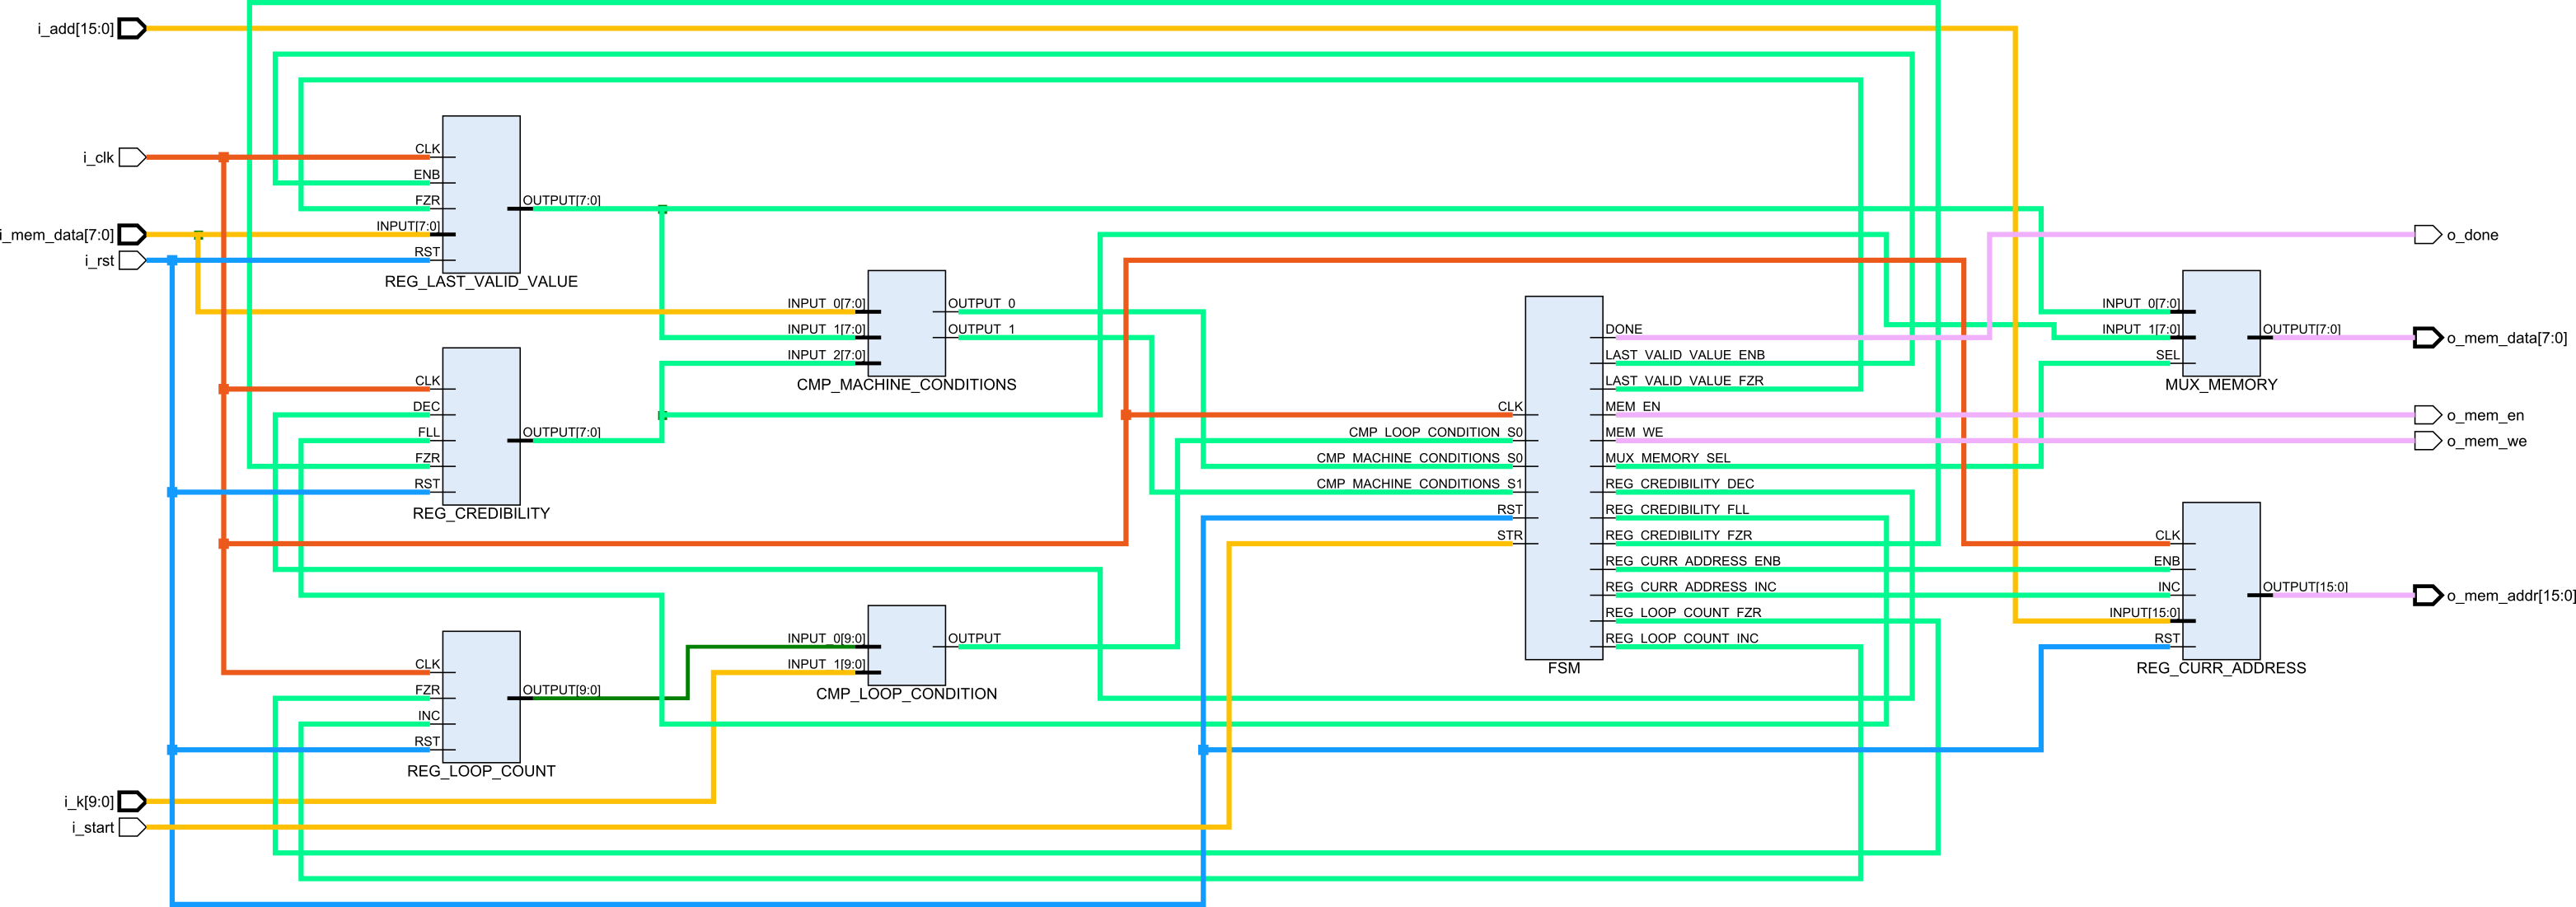
\includegraphics[width=1.3\textwidth]{resources/Datapath.png}
    }
\caption{Architettura del modulo}
\end{figure}

Le interconnessioni sono state evidenziate di colori diversi a seconda della loro funzione: in giallo i segnali d’ingresso, in rosso il segnale di clock, in blu il segnale di reset, in verde i segnali a uso interno e, in viola, i segnali d’uscita.

\subsubsection{Dettaglio dei vari componenti}

La presentazione dei componenti che compongono il datapath segue un ordine “funzionale”.

In caso di componenti sincroni, i pin di reset “RST” e di clock “CLK” vengono trascurati per semplicità: questi pin sono connessi direttamente ai segnali esterni e permettono l’inizializzazione dei moduli e la loro sincronizzazione.

\begin{itemize}
    \item \textbf{REG\_LAST\_VALID\_VALUE}: Registro PIPO sincrono a 8bit. Il modulo presenta un ingresso "INPUT" connesso al databus d’uscita della RAM in modo da poter salvare, quando la FSM porta "ENB" a 1, il valore della word W letto. La FSM può inoltre forzare a 0 il contenuto del modulo tramite forzante "FZR" per gestire il caso in cui l’elaborazione parta con W iniziale 0. L’uscita del componente "OUTPUT" è connessa – tramite il MUX – al databus d’ingresso della memoria per poter effettuare il rimpiazzo delle word non valide.
    \item \textbf{REG\_CREDIBILITY}: Registro contatore sincrono a 8bit. Viene utilizzato per memorizzare il valore di credibility C durante l’elaborazione. La FSM può decrementare il contenuto del modulo, di una unità, attraverso il pin "DEC" (l’underflow non è previsto, eventuali decrementi sotto lo 0 vengono ignorati) o forzare il componente a 31 tramite "FLL" o a 0 tramite "FRZ". L’uscita del registro "OUTPUT" è connessa al databus d’ingresso dalla RAM – tramite il MUX – per poter scrivere C in memoria.
    \item \textbf{MUX\_MEMORY}: Mux asincrono a 8bit da due canali. Viene utilizzato per connettere, a seconda del valore sul pin "SEL", le uscite di REG\_LAST\_VALID\_VALUE e REG\_CREDIBILITY (connesse rispettivamente a "INPUT\_0" e "INPUT\_1") al databus d’ingresso della RAM (connesso a "OUTPUT").
    \item \textbf{REG\_LOOP\_COUNT}: Registro contatore sincrono a 10bit. Memorizza il numero di iterazioni compiute. La FSM può incrementare, di una unità per volta, il valore memorizzato nel modulo tramite il pin "INC" (l’overflow non è consentito, incrementi sopra 1023 vengono ignorati) oppure può forzarne il contenuto a 0 mediante "FZR". L’uscita "OUTPUT" del registro è connesso al modulo CMP\_LOOP\_CONDITION che verrà discusso in seguito.
    \item \textbf{REG\_CURR\_ADDR}: Registro contatore sincrono a 16bit. Contiene al suo interno l’indirizzo della RAM in analisi in ogni fase del processo. Il componente ha un ingresso "INPUT" connesso direttamente al bus "i\_add" dell’entità e, quando richiesto dalla FSM, mediante il pin "ENB", l’indirizzo iniziale viene memorizzato. La FSM potrà poi incrementare, in maniera atomica, questo valore portando alto il pin "INC". L’uscita "OUTPUT" del modulo è connessa all’addressbus della RAM.
    \item \textbf{CMP\_MACHINE\_CONDITIONS}: Modulo comparatore asincrono usato come, abusando di questo termine, "branching unit" primaria della FSM. Le sue uscite sono connesse alla FSM: "OUTPUT\_0" (singolo pin) è 1 se e solo se "INPUT\_0" (vettore binario) è 0; essendo "INPUT\_0" connesso al databus d’uscita della RAM permette di sapere se il valore letto dalla memoria è valido. Allo stesso modo, "OUTPUT\_1" è 1 se e solo se sia "INPUT\_1" che "INPUT\_2" sono entrambi diversi da 0: per come è connesso il componente, quindi, permette di sapere se sia REG\_LAST\_VALID\_VALUE che REG\_CREDIBILITY sono entrambi nulli.
    \item \textbf{CMP\_LOOP\_CONDITION}: Modulo comparatore asincrono. La sua uscita "OUTPUT" permette di informare la FSM se REG\_LOOP\_COUNT, "INPUT\_0" ha raggiunto "i\_k", "INPUT\_1"; in tale condizione è necessario interrompere l’elaborazione.
\end{itemize}

\subsubsection{Dettaglio della FSM} % TODO (Pietro)
La FSM è il modulo che ha il controllo di tutti gli altri componenti: le sue uscite pilotano i vari pin di servizio degli altri costituenti mentre i suoi ingressi sono connessi alle due “branching unit” che controllano le transizioni di stato.
La macchina ha, inoltre, connessioni dirette con l’esterno. Considerando gli input troviamo: “STR" che avvia l'elaborazione e "RST" segnale asincrono di reset. Come output si trovano: “MEM\_WE" segnale di scrittura della memoria, “MEM\_EN" segnale di abilitazione della RAM e “DONE" che comunica il termine dell'elaborazione.

Segue descrizione degli stati:
%% MARKER
%inserire anche gli stati di wait. Sono inutili a livello logico??
\begin{enumerate}
    \item {\bf STARTING\_POINT}: Stato iniziale nel quale si posiziona la FSM in caso di reset o alla fine di una elaborazione. Non ha funzioni specifiche associate e non produce uscite. Quando viene dato il segnale di "i\_start" la macchina si porta in RESET\_REGISTERS, altrimenti permane in questo stato.
    \item {\bf RESET\_REGISTERS}: Per preparare i registri a una nuova elaborazione, imposta \\ REG\_LAST\_VALID\_VALUE, REG\_CREDIBILITY e REG\_LOOP\_COUNT a 0 utilizzando il segnale "FRZ". Inoltre, utilizza il segnale "ENB" per salvare l'indirizzo fornito da "i\_k" nel registro REG\_CURR\_ADDR. Dopo questa operazione, lo stato passa a CHECK\_LOOP\_CONDITION.
    \item {\bf CHECK\_LOOP\_CONDITION}: Introduce uno "stato dummy", che 'spreca' un ciclo di clock. Consente di sincronizzare il componente con la memoria. Attendendo che la memoria fornisca il contenuto dell'indirizzo salvato in REG\_CURR\_ADDR sull'uscita, permette ai moduli comparatori di generare l'output che guiderà le transizioni. Questo stato non genera alcuna uscita e viene seguito da CHECK\_LOOP\_CONDITION\_WM.
    \item {\bf CHECK\_LOOP\_CONDITION\_WM}: Se la macchina ha processato tutte le K word W (CMP\_LOOP\_CONDITION\_S0 = '1'), l'elaborazione termina e la macchina si sposta nello stato ELABORATION\_ENDED. Tuttavia, se è ancora in fase di lavoro e la word W da processare è pari a 0 (CMP\_MACHINE\_CONDITIONS\_S0 = '1'), diventa necessario intervenire con la procedura di sostituzione. Si porta nello stato RAM\_TO\_REG\_LVV. In alternativa, se la word W è valida (CMP\_MACHINE\_CONDITIONS\_S0 = '0'), la macchina a stati salva la nuova parola per futura referenza e aggiorna il valore di credibilità. Questa procedura inizia portandosi nello stato FILL\_CREDIBILITY. Anche questo stato è privo di uscite.
    \begin{itemize}
        \item Caso W valido:
            \begin{enumerate}
                \item {\bf FILL\_CREDIBILITY}: Reimposta il valore di credibilty a 31 (credibilità massima) portando a 1 il segnale "FLL" del registro preposto. Segue\\RAM\_TO\_REG\_LVV.
                \item {\bf RAM\_TO\_REG\_LVV}: Stato di sincronizzazione. In questo stato si attiva il segnale "ENB" di REG\_LAST\_VALID\_VALUE per salvare nel registro la parola, valida, letta dalla memoria. Segue RAM\_TO\_REG\_LVV\_WM.
                \item {\bf RAM\_TO\_REG\_LVV\_WM}: Alza il segnale "ENB" di \\REG\_LAST\_VALID\_VALUE; W è ora nel registro. Segue \\INCREASE\_ADDRESS\_COUNTER; incrementando il contatore degli indirizzi, si posiziona la memoria sull'indirizzo contenente C. Poiché W è valida, sovrascrive il contenuto dell'indirizzo con il valore 31, ottenuto dal registro \\REG\_CREDIBILITY precedentemente forzato, copiandolo in RAM.
             \end{enumerate}
        \item Caso W non valido:
        \begin{enumerate}
                \item {\bf REG\_TO\_RAM\_LVV}: Sovrascrive, al posto dello 0 presente in memoria, l'ultima parola W valida letta. Per fare ciò porta a '1' il segnale di WRITE\_ENABLE della memoria ("o\_mem\_we"). Se sia l'ultima W valida che C sono diversi da 0 (CMP\_MACHINE\_CONDITIONS\_S1 = '1'), segue DECREASE\_CREDIBILITY; altrimenti, il decremento è inutile e si passa direttamente a \\INCREASE\_ADDRESS\_COUNTER.
                \item{\bf DECREASE\_CREDIBILITY}: Decrementa di una unità il registro REG CREDIBILITY. Per fare questo la FSM alza il segnale "DEC" del registro. Segue INCREASE\_ADDRESS\_COUNTER.
        \end{enumerate}
    \end{itemize}
    \item {\bf INCREASE\_ADDRESS\_COUNTER}: Incrementa di una unità il valore contenuto nel registro REG\_CURR\_ADDR dove è salvato l'indirizzo corrente da dove leggere/scrivere in memoria. Per fare ciò l'uscita "INC" del registro è alzata a '1'. Segue REG\_TO\_RAM\_CC.
    \item {\bf REG\_TO\_RAM\_CC}: Scrive in memoria il valore corrente di credibilità: il valore contenuto nel registro REG\_CREDIBILITY viene copiato in RAM. Per permettere la scrittura è alzato a '1' il segnale di WRITE\_ENABLE; inoltre, viene modificato il segnale di controllo sul MUX per instradare l'uscita dal modulo sul databus di scrittura della RAM. Segue INCREASE\_ADDRESS\_COUNTER.
    \item {\bf INCREASE\_ADDRESS\_LOOP\_COUNTER}: Incrementa di una unità il valore contenuto nel registro REG\_CURR\_ADDR, dove è salvato l'indirizzo corrente dove leggere/scrivere in memoria. Per fare ciò l'uscita INCREASE\_ADDRESS\_COUNTER è alzata a '1'. Contemporaneamente aumenta di una unità anche il registro REG\_LOOP\_COUNT alzando l'uscita REG\_LOOP\_COUNT\_INC.
    \item {\bf ELABORATION\_ENDED}: Porta a zero il valore del segnale DONE, comunicando il termine dell'esecuzione. Quando il segnale di input "STR" è riporto a zero, si riporta a STARTING\_POINT, pronta per una nuova esecuzione; altrimenti la macchina rimane in questo stato.
\end{enumerate}

La dicitura "RAM\_TO\_REG" riporta una operazione di lettura dalla memoria e salvataggio del contenuto in un registro, mentre "REG\_TO\_RAM" è una operazione di scrittura in memoria di un dato contenuto in un registro.

L'automa è una macchina di Moore: le uscite della FSM sono determinate in funzione dello stato corrente e non dipendono dai segnali d'ingresso.

Nella pagina successiva segue il diagramma degli stati della macchina. Le condizioni di branching, per semplificare la lettura, sono espresse "a livello semantico"; nella descrizione testuale sono comunque riportati i segnali interessati.

% 2.2.2. Dettaglio della FSM -> Tabella degli stati (forma grafica e/o tabellare)
\begin{figure}[H] 
\centering
\caption{Macchina a stati}
\begin{tikzpicture} [shorten >= 2pt, node distance = 3cm,on grid,auto, align=center, every state/.style={fill=Cyan!10}]
    \node[state, initial, align=center] (q0)                                            {Starting\\Point}; 
    \node[state] (q1)  [right= 4cm of q0, align=center]                                 {Reset\\Registers};
    \node[state] (q11) [below = 2.5cm of q1, align=center]                              {Check\\Loop\\Condition};
    \node[state] (q2)  [below = 3cm of q11, align=center]                               {Check\\Loop\\Condition WM};
    \node[state] (q3)  [below = 4cm of q2,  xshift = -2cm, align=center]                {Fill\\Credibility};
    \node[state] (q4)  [below = 5cm of q3, xshift=-1cm]                               {RamToReg\\LVV};
    \node[state] (q13) [below = 0cm of q4, xshift= 3.5cm]                               {RamToReg\\LVV WM};

    %parte a destra
    \node[state](q12) [below = 3.5cm of q2, xshift= 4cm]               {RegToRam\\LVV};
    \node[state](q6) [below = 3cm of q12]                            {Decrease\\Credibility};
    \node[state](q7) [below = 3cm of q6]                             {Increase\\Address\\Counter};
    \node[state](q8) [below = 3cm of q7]                             {RegToRam\\CC};
    \node[state](q9) [right = 3cm of q8]                             {Increase\\Address\\Loop Counter};
    %parte sinistra
    \node[state](q10) [below = 0cm of q2, xshift= -6cm]              {Elaboration\\Ended};

    \path[->] (q0) edge node {$i\_start = 1$} (q1)
              (q1) edge node {} (q11)
              (q11) edge node {} (q2)
              (q2) edge node [anchor= east]{$W \neq 0$} (q3)
              (q3) edge [bend right=10] node {} (q4)
              (q13) edge node {} (q7)
              (q2) edge [bend left=10] node[xshift=-0.2cm] {$W = 0$} (q12)
              (q12) edge node {} (q6)              
              (q12) edge node[anchor=east] {$C \neq 0 \wedge LVV \neq 0$} (q6)
              (q6) edge node {} (q7)
              (q7) edge node {} (q8)              
              (q8) edge node {} (q9)
              (q10) edge [bend left=10] node {$i\_start = 0$}(q0) 
              (q2) edge [bend right=10] node[anchor=south, yshift=0.5cm, xshift = -0.1cm] {Elaborate tutte le K parole} (q10)
              (q10) edge[loop below] node{$i\_start = 1$}(q10)
              (q9) edge [bend right=80] node {} (q2)
              (q12) edge [bend left=50] node{$C = 0$} (q7)    
              (q4) edge node{} (q13)      
              (q0) edge [loop above] node{$i\_start = 0$} (q0);
\end{tikzpicture}
\end{figure}

\newpage

\section{Risultati sperimentali}
\subsection{Testbench}
Per quanto riguarda il testing del modello abbiamo validato la macchina contro i seguenti testbench:

\begin{table}[H]
\centerline{
\resizebox{1.1\textwidth}{!}{%
\begin{tabular}{|l|l|l|l|l|l|}
\hline
\textbf{TB}                               & \textbf{K} & \textbf{Sim. Behavioural} & \textbf{Tempo (ns)} & \textbf{Sim. Post-synthesis} & \textbf{Tempo (ns)} \\ \hline
ORIGINAL\_TB                              & 14         & PASSED                    & 2890                & PASSED                       & 2890                \\ \hline
EXAMPLE\_1                                & 10         & PASSED                    & 2150                & PASSED                       & 2150                \\ \hline
EXAMPLE\_2                                & 35         & PASSED                    & 6490                & PASSED                       & 6490                \\ \hline
EXAMPLE\_3                                & 33         & PASSED                    & 6290                & PASSED                       & 6290                \\ \hline
EXAMPLE\_4                                & 10         & PASSED                    & 2070                & PASSED                       & 2070                \\ \hline
EXAMPLE\_5                                & 16         & PASSED                    & 3430                & PASSED                       & 3430                \\ \hline
OTHERS\_ALL\_ZEROS                        & 10         & PASSED                    & 1830                & PASSED                       & 1830                \\ \hline
OTHERS\_HALF\_ZEROS                       & 10         & PASSED                    & 1950                & PASSED                       & 1950                \\ \hline
OTHERS\_CREDIBILITY\_FILL\_TO\_ZERO       & 41         & PASSED                    & 7450                & PASSED                       & 7450                \\ \hline
OTHERS\_K\_FAILURE                        & 0          & PASSED                    & 250                 & PASSED                       & 250                 \\ \hline
OTHERS\_MULTIPLE\_CONSECUTIVE\_EXECUTIONS & 36         & PASSED                    & 7430                & PASSED                       & 7430                \\ \hline
OTHERS\_RESET\_AND\_RESUME                & 16         & PASSED                    & 6330                & PASSED                       & 6330                \\ \hline
\end{tabular}%
}
}
\end{table}

\begin{itemize}
    \item \textbf{ORIGINAL\_TB}: Testbench messo a disposizione su WeBeep.
    \item \textbf{EXAMPLE\_1} fino a \textbf{EXAMPLE\_5}: Testbench, scritti a partire da quello d’esempio, che emulano gli esempi presenti nel file PDF di specifica.
    \item \textbf{OTHERS\_ALL\_ZEROS}: Controlla il funzionamento della macchina in risposta a una memoria di soli zeri.
    \item \textbf{OTHERS\_HALF\_ZEROS}: Controlla che la macchina, incaricata di processare una serie di valori che inizia per 0, sia in grado poi di comportarsi correttamente quando smette di incontrare valori nulli.
    \item \textbf{OTHERS\_CREDIBILITY\_FILL\_TO\_ZERO}: Viene chiesto alla macchina di processare una sequenza di word W lunga abbastanza da controllare se il meccanismo di protezione contro l’underflow della credibilità (il valore minimo della credibilità è 0) è correttamente gestito.
    \item \textbf{OTHERS\_K\_FAILURE}: Viene controllato che la macchina reagisca correttamente nel caso in cui parta un’esecuzione fornendo K=0.
    \item \textbf{OTHERS\_MULTIPLE\_CONSECUTIVE\_EXECUTIONS}: Controlla che la macchina sia in grado di eseguire correttamente esecuzioni consecutive senza necessitare di un reset tra le procedure.
    \item \textbf{OTHERS\_RESET\_AND\_RESUME}: Viene fatta partire una esecuzione ma, prima che questa possa finire, viene inviato un segnale di reset. Viene poi fatto ripartire il componente con gli stessi valori di K e ADD. La memoria viene poi controllata, considerando i nuovi valori.
\end{itemize}

Tutti i testbench che abbiamo scritto funzionano sia in pre- che in post-sintesi. Escludendo dalla statistica il TB OTHERS\_K\_FAILURE, dove $K=0$, il tempo medio richiesto dalla macchina per terminare il suo compito è circa pari a $\approx 200ns \cdot K$ (questo valore è solo indicativo visto che, a scopo di debug, nei TB sono spesso aggiunti ritardi per facilitare i controlli).

Avendo un'implementazione Python dell'algoritmo "eseguito", in senso lato, dalla macchina, siamo riusciti a sviluppare rapidamente un generatore automatico di TB. Tuttavia, è importante sottolineare che l'uso di test generati automaticamente presenta limitazioni in termini di coverage: questi test tendono a riprodurre scenari predefiniti e non sono in grado di esplorare in modo esaustivo tutte le possibili condizioni operative del componente.

\subsection{Report di sintesi}
Abbiamo sintetizzato il nostro progetto sulla scheda AMD Xilinx Artix-7 XC7A200TFBG484-1, come richiesto dal regolamento, e il footprint sulla scheda è minimo:

\begin{table}[H]
\centering
\begin{tabular}{|l|l|l|l|}
\hline
\textbf{Risorsa} & \textbf{Utilizzo} & \textbf{Disponibilità} & \textbf{\% Utilizzo} \\ \hline
LUT              & 68                & 133800                 & 0,05                 \\ \hline
FF               & 55                & 269200                 & 0,02                 \\ \hline
IO               & 64                & 285                    & 22,46                \\ \hline
BUFG             & 1                 & 32                     & 3,13                 \\ \hline
\end{tabular}
\end{table}

Scendendo maggiormente in dettaglio:

\begin{table}[H]
\centering
\begin{tabular}{|l|l|l|l|l|l|}
\hline
\textbf{Site Type}    & \textbf{Used} & \textbf{Fixed} & \textbf{Prohibited} & \textbf{Available} & \textbf{Util \%} \\ \hline
Slice LUTs            & 68            & 0              & 0                   & 134600             & 0,05           \\ \hline
LUT as Logic          & 68            & 0              & 0                   & 134600             & 0,05           \\ \hline
LUT as Memory         & 0             & 0              & 0                   & 46200              & 0,00           \\ \hline
Slice Registers       & 55            & 0              & 0                   & 269200             & 0,02           \\ \hline
Register as Flip Flop & 55            & 0              & 0                   & 269200             & 0,02           \\ \hline
Register as Latch     & 0             & 0              & 0                   & 269200             & 0,00           \\ \hline
F7 Muxes              & 0             & 0              & 0                   & 67300              & 0,00           \\ \hline
F8 Muxes              & 0             & 0              & 0                   & 33650              & 0,00           \\ \hline
\end{tabular}
\end{table}

Dai report si conclude che il nostro design utilizza solo una minima frazione delle risorse messe a disposizione dalla scheda e che il nostro sorgente VHDL non utilizza alcun latch. 

\subsection{Report timing}

Il regolamento prevedeva un time constraint di 20ns. Siamo riusciti a soddisfare questo requisito; gli strumenti interni a Vivado riportano:

\centerline{Slack (MET): 16.200ns (required time - arrival time)}

Lo slack è quindi contenuto nel range di ammissibilità.

\section{Conclusioni}
Abbiamo implementato, in linguaggio VHDL, un modulo capace di gestire operazioni di scrittura e lettura su una memoria esterna.

Il modulo soddisfa tutte le specifiche progettuali e ha superato una serie di test automatici, generati in Python, e manuali per garantirne l'affidabilità, anche nei casi più complessi.

Questo progetto ci ha fornito una preziosa introduzione pratica alla progettazione e verifica di sistemi digitali complessi, aprendo la strada a ulteriori opportunità di apprendimento e sviluppo.

\newpage
\thispagestyle{empty}
\begin{landscape}
    \begin{figure}
        \centering
        \centerline{
        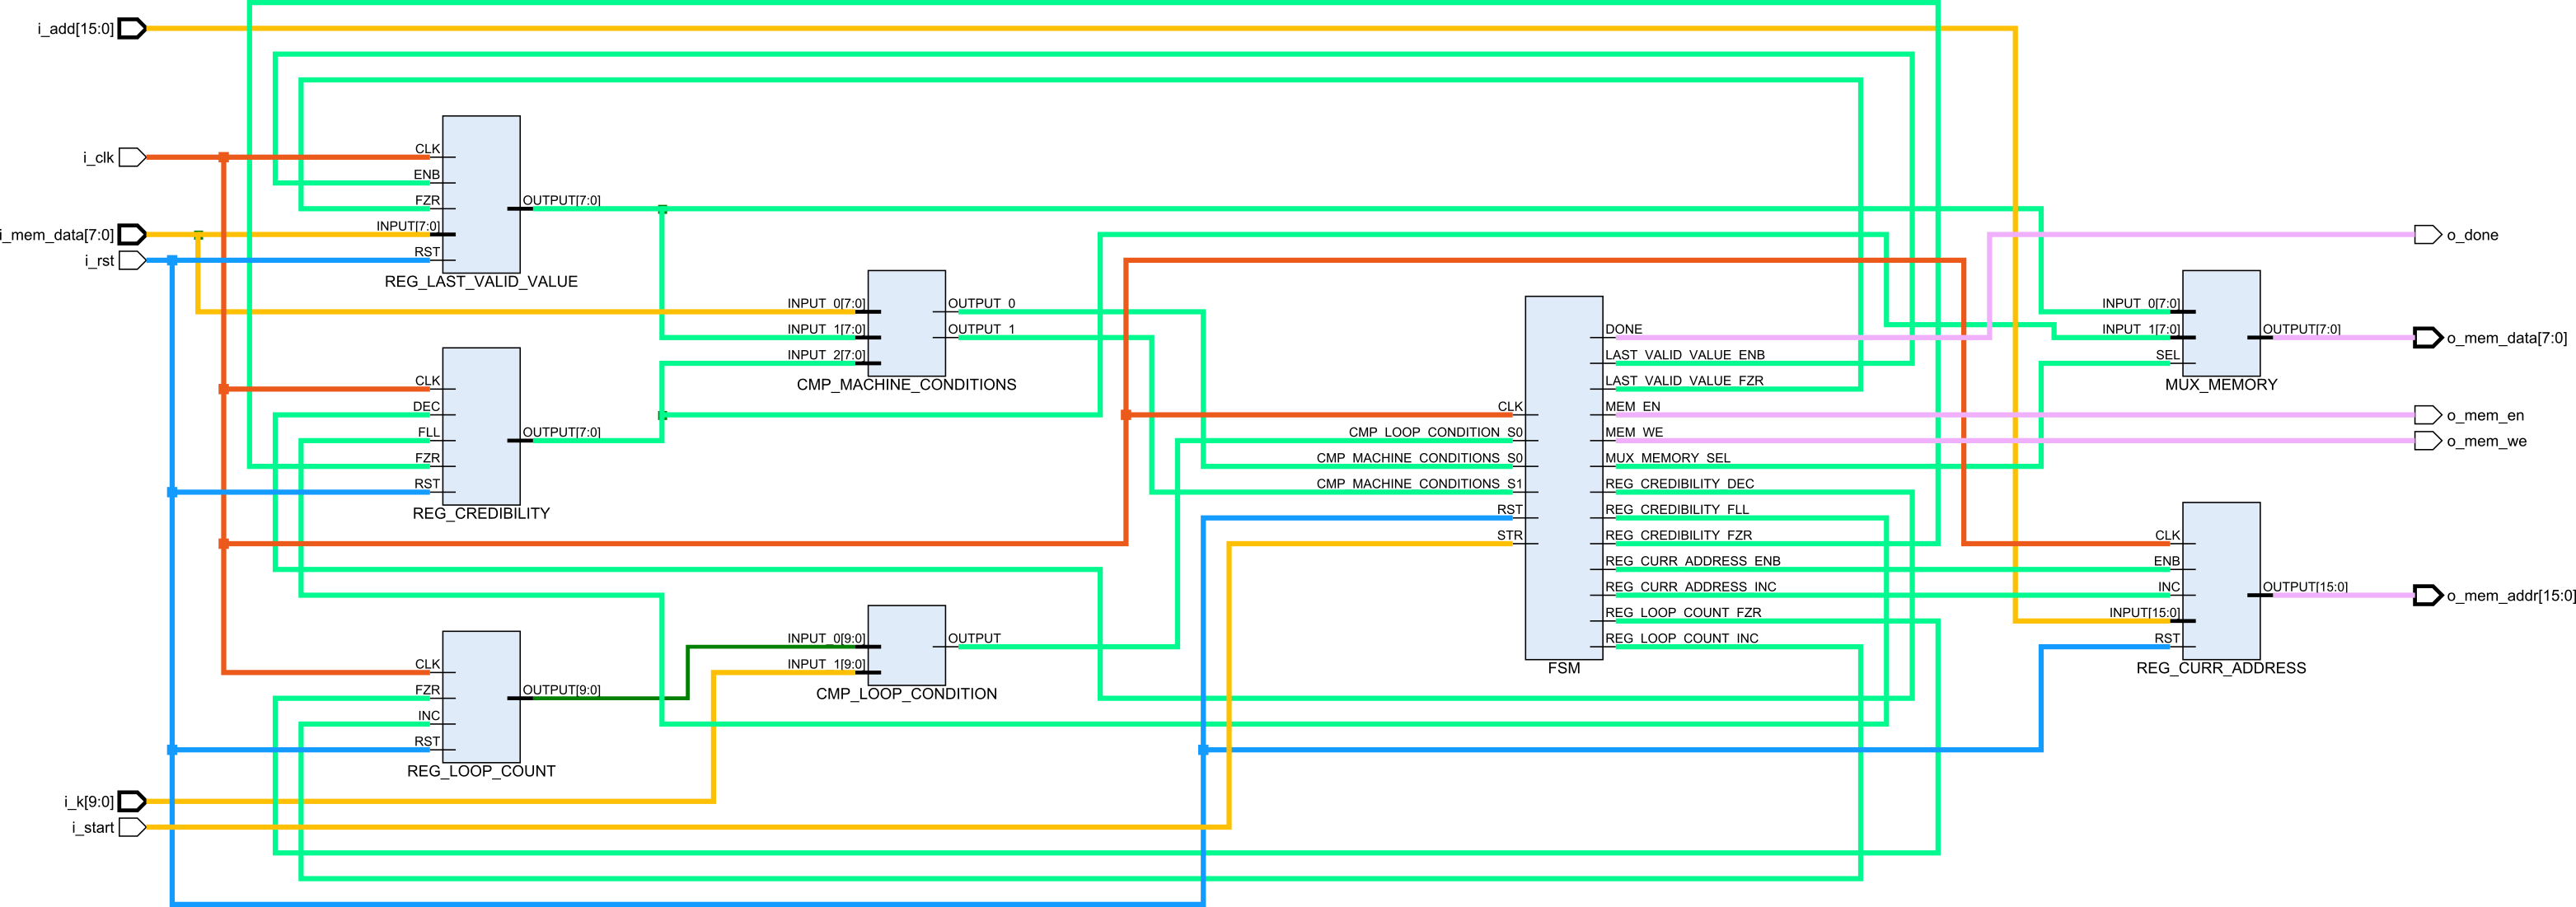
\includegraphics[width=29cm]{resources/Datapath.png}
        }
    \end{figure}
\end{landscape}

\end{document}
